
% die Standard-Dokumentenklasse
\documentclass[11pt,a4paper]{article} %% 1.Ebene = chapter, headings

% input encoding, font encoding, outline font
\usepackage[utf8]{inputenc} 
\usepackage[T1]{fontenc} 
\usepackage{lmodern}
\usepackage{tcolorbox}
% Sprache
\usepackage[german]{babel}
\usepackage[section]{placeins}

% Absatzformatierung
\setlength{\parindent}{0pt}
\setlength{\parskip}{1ex plus 0.5ex minus 0.5ex}

% erweiterte mathematische Symbole
\usepackage{amsmath} 

% für Abbildungen
\usepackage{graphicx} 

% für Tabellen
\usepackage{booktabs}

% für Hyperlinks
\usepackage[colorlinks]{hyperref}
\graphicspath{}




\begin{document}

	

{
	\centering 
	\large 
	Physiklabor für Anfänger*innen \\
	Ferienpraktikum im Sommersemester 2018 \\[4mm]
	\textbf{\LARGE 
		Versuch 31: Mischungsmethode in der Kalorimetrie
	} \\[3mm]
	(durchgeführt am 12.09.2018 bei Nico Strauß) \\
	Ye Joon Kim, Marouan Zouari\\
	\today \\[10mm]
}

\section{Einleitung}
Die Wärmekapazität ist das Verhältnis der einem Körper zugeführte Wärme zu seinem Temperaturerhöhung. Bei Experimenten mit Kalorimeter ist es oft hilfreich die Wärmekapazität des Kalorimeters zu kennen, damit bessere Ergebnisse bekommen werden können. 

Aber es gibt auch Ausnahme, wobei die Temperatur trotz Energiezufuhr sich nicht erhöht. Bei Phasenübergänge verursacht die Aufnahme oder Abgabe von Wärme keine Temperaturänderung. Die latente Wärme quantifiziert die Menge Wärme, die bei einem Phasenübergang aufgenommen oder abgegeben wird, ohne die Temperatur zu ändern. Insbesondere ist die latente Wärme beim Schmelzen auch als Schmelzwärme bezeichnet. 


\section{Ziel des Versuchs}
Das Ziel dieses Versuchs ist es, mit der Mischungsmethode verschiedene physikalische Werte zu bestimmen. In dem ersten Versuchsteil wird die Mischungsmethode verwendet um die Wärmekapazität eines Kalorimeters zu bestimmen. In dem zweiten Teil wird die Schmelzwärme von Eis bestimmt. 

\section{Aufbau}
\begin{figure}
	\centering
	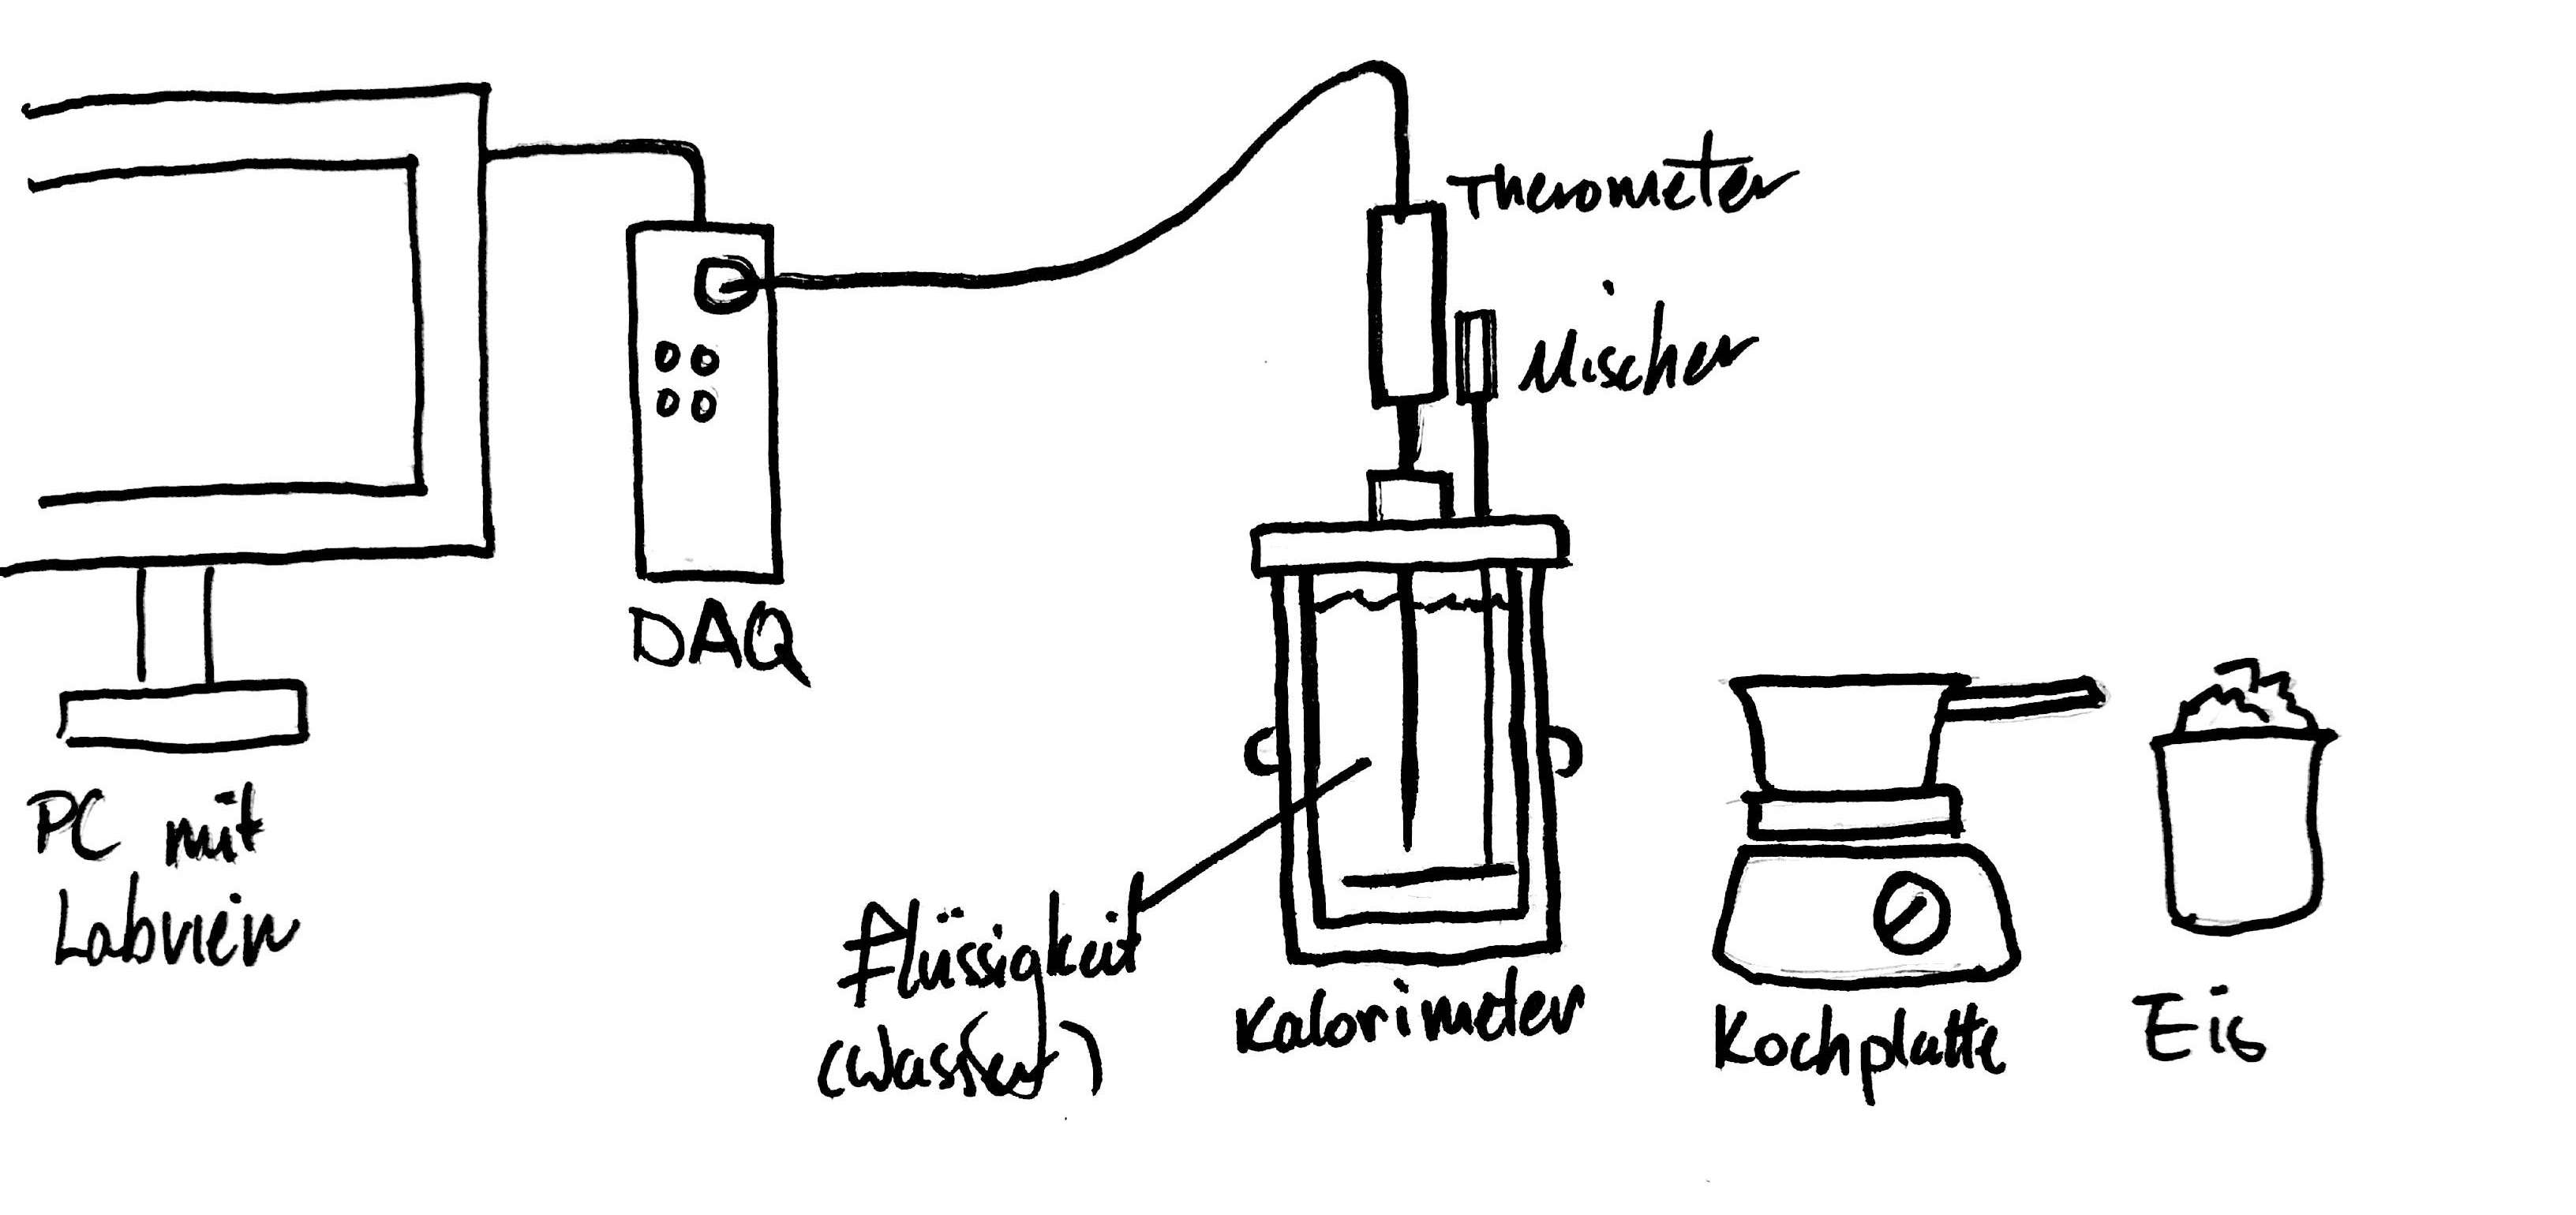
\includegraphics[width=\linewidth]{Abb3}
	\caption{Aufbau zu beiden Versuchsteilen}
\end{figure}

\section{Auswertung und Fehleranalyse}

\subsection{Zur Kalibrierung}
Zur Kalibrierung wurde Eis und kochendes Wasser verwendet. Zuerst wurde die Temperatur von Eis mit dem Thermometer gemessen. Für die akkurate Messung von 0 $^\circ$C wurde es gewartet, bis das Eis ein bisschen geschmolzen war, damit eine Eis-Wasser Mischung entstanden war. Die Abweichung von 0 $^\circ$C wurde dann von dem Messwert subtrahiert, damit der Apparat 0 $^\circ$C genau misst. Dann wurde die Temperatur des kochendes Wasser gemessen. Sei $T$ der gemessene Wert. Die Messwerte wurden dann mit $\frac{100}{T}$ multipliziert, um die Messungen zu "Skalieren". Dadurch sind die Messwerte für 0 $^\circ$C und 100 $^\circ$C akkurat, und deshalb der Thermometer kalibriert. 

\subsection{1. Versuchsteil: Bestimmung der Wärmekapazität des Kalorimeters}

Zur Bestimmung der Wärmekapazität des Kalorimeters wird die folgende Wärmeenergiebilanz benutzt:
\begin{equation}
 \Gamma_\textrm{Kal} = c_\textrm{W}(m_\textrm{k}\beta-m_\textrm{h})  \quad \textrm{mit} \quad \beta = \frac{T_M-T_k}{T_h-T_M}
\end{equation}
\begin{table}[h]
	\centering
	\begin{tabular*}{0.99\textwidth}{@{\extracolsep{\fill}}cccccc}
		\toprule
		Messreihe & $T_M$ & $\Delta T_M$  \\
		& $^\circ$ C & $^\circ$ C \\
		1 & 43 & 2  \\
		2 & 23 & 2 \\
		3 & 61 & 2 \\
		\bottomrule
	\end{tabular*}
	\caption{Die Berechneten Mischungstemperaturen und deren Unsicherheiten.}
	\label{tabelle}
\end{table}


Für das Extrapolationsverfahren wurde das Photoshop\textregistered Programm von Adobe   benutzt. Eine Kurve wurde mit dem Pen-tool gezeichnet, die den Temperaturverlauf modelliert. Dann wurde eine Senkrechte Linie eingezeichnet nach dem Zeitpunkt, wo das kalte Wasser in das Kalorimeter gegossen wurde. Mit dem Lasso-Tool kann die Gebiete zwischen die Kurve und die Linie ausgewählt und deren Flächen berechnet werden. Die Linie wurde bewegt, bis beide Gebiete schätzungsweise gleich waren. 
\begin{figure}[h]
\centering
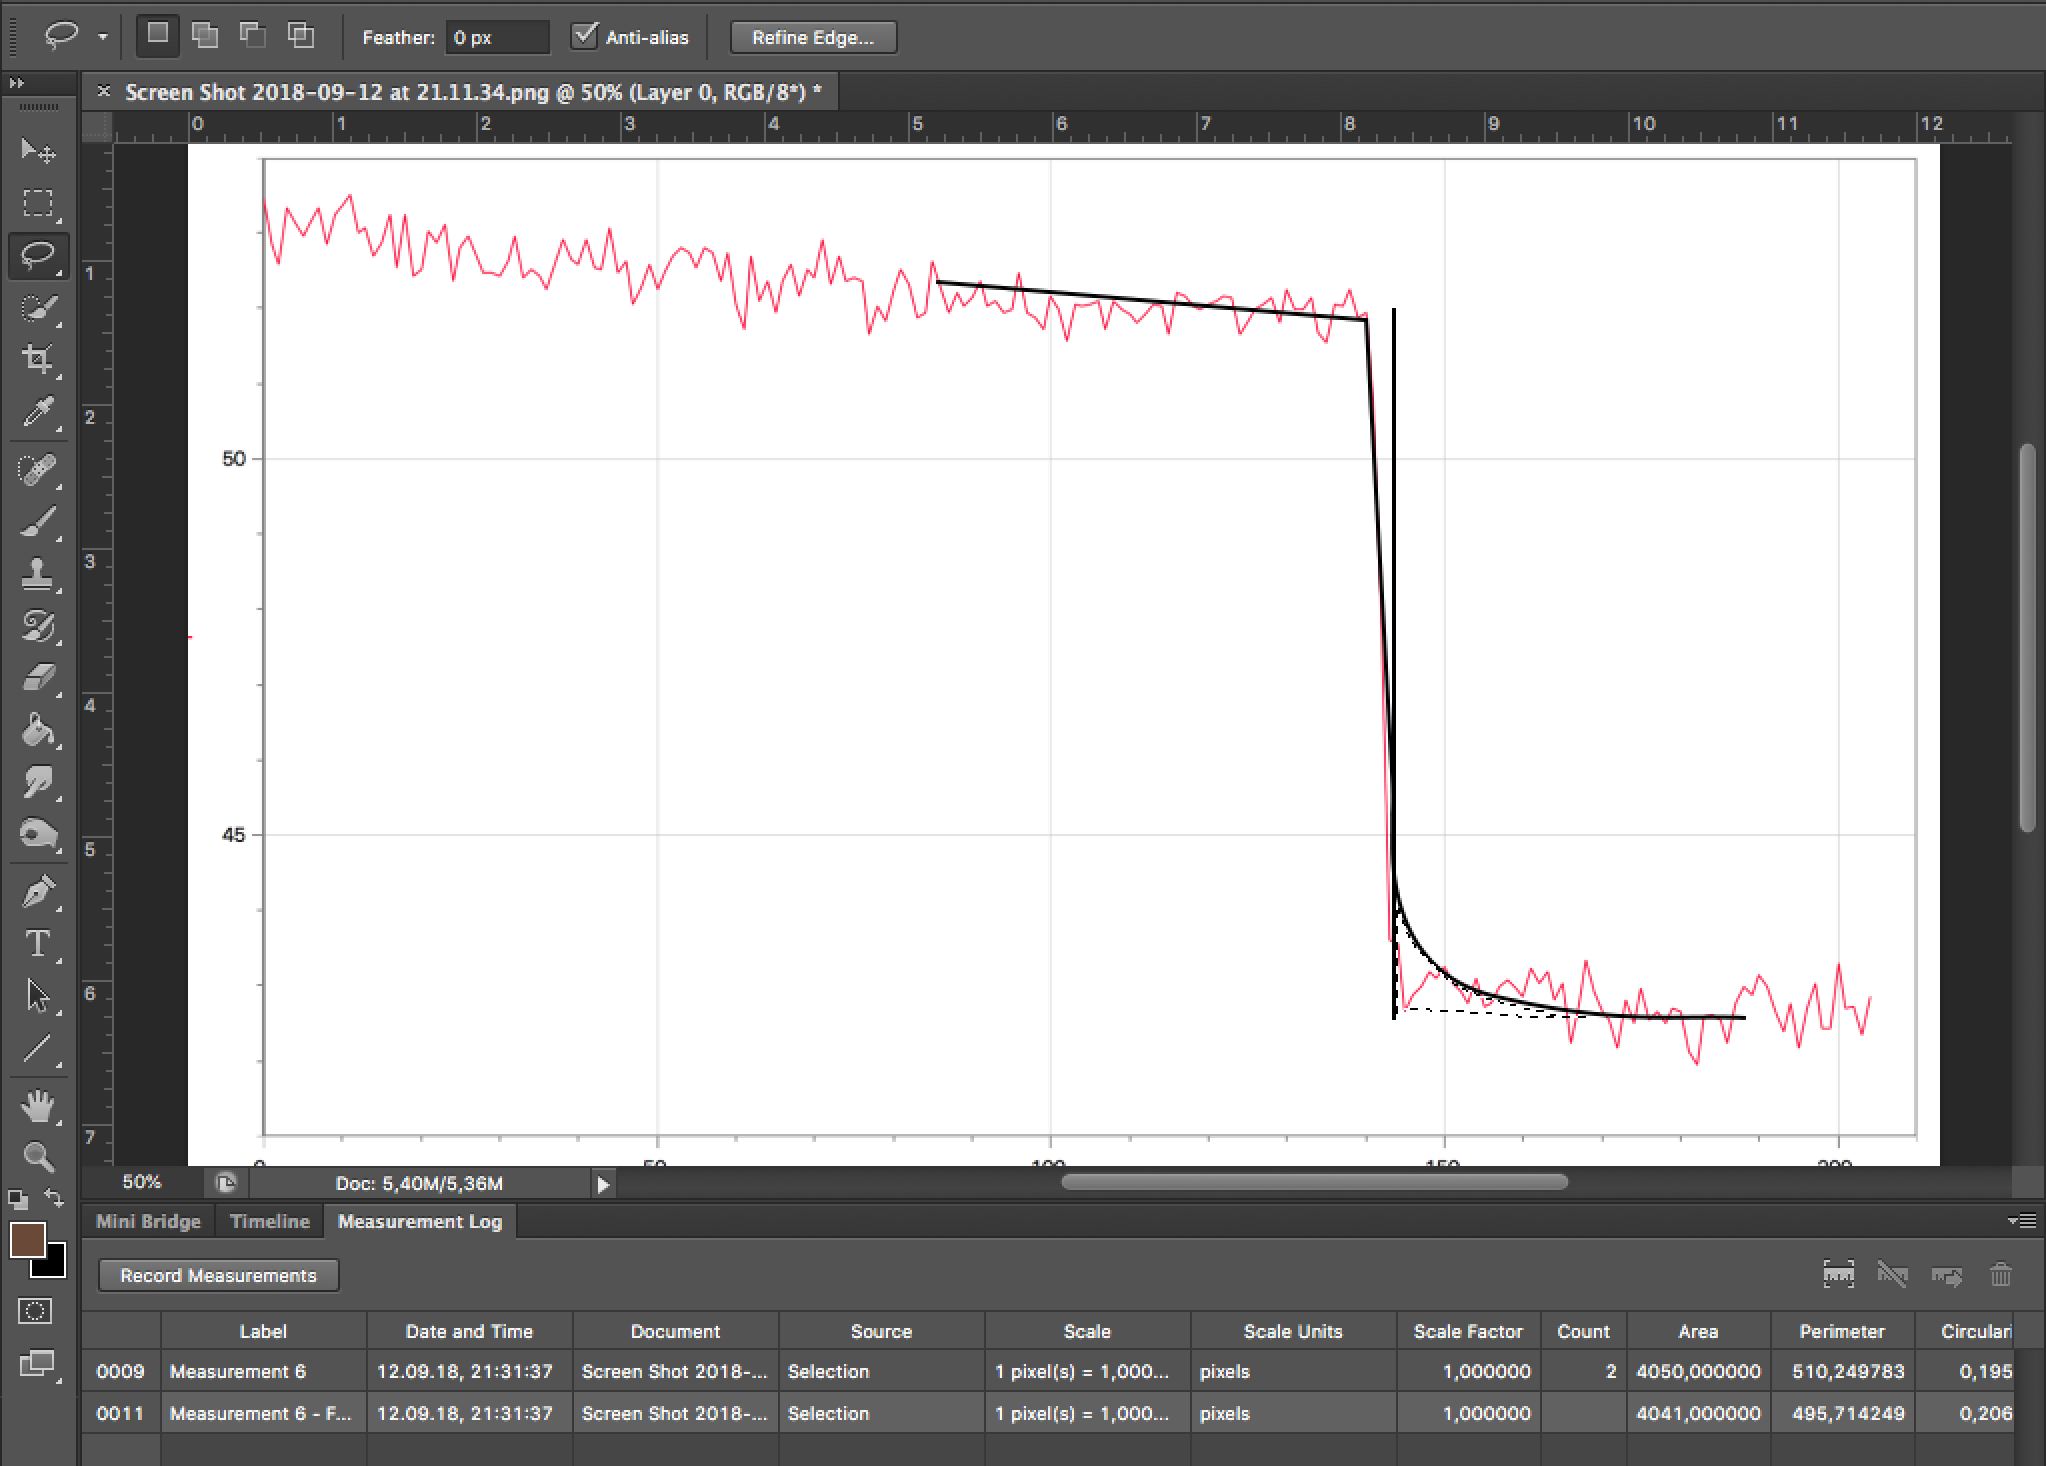
\includegraphics[width=\linewidth]{Abb1}
\caption{Benutzung von Photoshop um die Fläche von beide Gebiete vor und nach der Senkrechte Strecke}

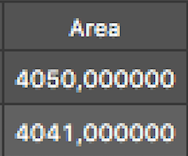
\includegraphics{Abb2}
\caption{Vergleich der Flächen beider Gebiete. (Einheiten in Pixels)}
\end{figure}
\FloatBarrier
Die Unsicherheiten bei der Temperatur wurden von dem Diagramm abgeschätzt. 
	
Jetzt lassen sich die Werte für $\Gamma_\textrm{Kal}$ mit den Werten für $T_h$, $T_k$, $m_k$, und $m_h$ bestimmen. 

\begin{table}[h]
	\centering
	\begin{tabular*}{0.99\textwidth}{@{\extracolsep{\fill}}cccccc}
		\toprule
		Messreihe & $\Gamma_\textrm{Kal}$ & $\Delta \Gamma_\textrm{Kal}$  \\
		& J / K & J/ K\\
		1 & 107 & 95  \\
		2 & 126 & 176 \\
		3 & 15 & 73 \\
		\bottomrule
	\end{tabular*}
	\caption{Die Wärmekapazität des Kalorimeters und deren Unsicherheiten.}
	\label{tabelle3}
\end{table}

\begin{tcolorbox}[colback=white]
Für die Berechnung der Unsicherheit wurden die Gauß'sche Fehlerfortpflanzung mit:
$$f(m_k, m_h, T_M, T_k, T_h) = c_\textrm{W}(m_\textrm{k} \frac{T_M-T_k}{T_h-T_M} -m_\textrm{h}) $$
$$ \frac{\partial f}{\partial m_k} = c_W\frac{T_M-T_k}{T_h-T_M}$$
$$ \frac{\partial f}{\partial m_h} = c_W$$
$$ \frac{\partial f}{\partial T_h} = -c_W m_k \frac{T_M - T_k}{(T_h-T_M)^2} $$
$$ \frac{\partial f}{\partial T_k} = \frac{-c_W m_k}{T_h-T_M} $$
$$ \frac{\partial f}{\partial T_M} = c_W m_k \frac{T_h-T_k}{(T_M-T_h)^2} $$
benutzt. Aber da $\frac{\partial f}{\partial T_M} \Delta T_M$, $\frac{\partial f}{\partial T_h} \Delta T_h$ und $\frac{\partial f}{\partial T_k} \Delta T_k$ überwiegend größer als die anderen Terme (mindestens dreimal größer) sind, wurden die Unsicherheit berechnet als:
$$\Delta \Gamma_\textrm{Kal} = \sqrt{(\frac{\partial f}{\partial T_M} \Delta T_M)^2+(\frac{\partial f}{\partial T_h} \Delta T_h)^2+(\frac{\partial f}{\partial T_k} \Delta T_k)^2}$$

\end{tcolorbox}

Der Mittelwert und seine Unsicherheit (Standardabweichung) lauten:
$$(83 \pm 60 ) \textrm{J / K}$$

\subsection{2. Versuchsteil: Bestimmung der Schmelzwärme von Eis}

Die Schmelzwärme von Eis (mit $q_\textrm{Eis}$ bezeichnet ) lässt mit der folgenden Formel bestimmen:


\begin{equation}
q_\textrm{Eis} = \frac{(m_W c_W + \Gamma_\textrm{Kal})(T_W - T_M) - m_\textrm{Eis} c_W(T_M - T_\textrm{Eis})}{m_\textrm{Eis}}
\end{equation}

Die Werte für $T_M$ lassen sich wiederum mit dem obigen Extrapolationsverfahren (in Teil 4.1) bestimmen. 

\begin{table}[h]
	\centering
	\begin{tabular*}{0.99\textwidth}{@{\extracolsep{\fill}}cccccc}
		\toprule
		Messreihe & $T_M$ & $\Delta T_M$  \\
		& $^\circ$ C & $^\circ$ C \\
		1 & 25 & 2  \\
		2 & 32 & 2 \\
		3 & 38 & 2 \\
		\bottomrule
	\end{tabular*}
	\caption{Die Mischungstemperaturen und deren Unsicherheiten}
	\label{tabelle2}
\end{table}

und die Werte für $T_M$ eingesetzt in Formel (2) liefern:

\begin{table}[h]
	\centering
	\begin{tabular*}{0.99\textwidth}{@{\extracolsep{\fill}}cccccc}
		\toprule
		Messreihe & $q_\textrm{Eis}$ & $\Delta q_\textrm{Eis}$  \\
		& J / kg & J / kg \\
		1 & 668400 & 10000  \\
		2 & 110000 & 96000 \\
		3 & 21000 & 22000 \\
		\bottomrule
	\end{tabular*}
	\caption{Die berechneten Werte für die Schmelzwärme von Eis}
	\label{tabelle4}
\end{table}

\begin{tcolorbox}[colback=white]
Für die Unsicherheiten wurde die Gauß'sche Fehlerfortpflanzung benutzt. Mit:
$$f(m_W,\Gamma_\textrm{Kal},T_W, T_M, m_\textrm{Eis}) $$ 
$$ = \frac{(m_W c_W + \Gamma_\textrm{Kal})(T_W - T_M) - m_\textrm{Eis} c_W(T_M - T_\textrm{Eis})}{m_\textrm{Eis}} $$
sind:
$$ \frac{\partial f}{\partial m_W} = \frac{c_W(T_W-T_M)}{m_\textrm{Eis}}$$
$$ \frac{\partial f}{\partial \Gamma_\textrm{Kal}} = \frac{T_W-T_M}{m_\textrm{Eis}}$$
$$ \frac{\partial f}{\partial T_W} = \frac{m_W c_W + \Gamma_\textrm{Kal}}{m_\textrm{Eis} }$$
$$ \frac{\partial f}{\partial T_M} = \frac{m_W c_W + \Gamma_\textrm{Kal} - m_\textrm{Eis} c_W}{m_\textrm{Eis}} $$
$$\frac{\partial f}{\partial m_\textrm{Eis}} = \frac{m_W c_W + \Gamma_\textrm{Kal}}{m_\textrm{Eis}^2}$$
Aber da der Betrag von $\frac{\partial f}{\partial \Gamma_\textrm{Kal}} \Delta \Gamma_\textrm{Kal}$ mindestens dreimal größer war als alle andere Beträge, wurde die anderen Beträge vernachlässigt. 
Die Unsicherheiten der Werte für $q_\textrm{Eis}$ sind dann:
$$\Delta q_\textrm{Eis} = \frac{\partial f}{\partial \Gamma_\textrm{Kal}} \Delta \Gamma_\textrm{Kal} $$


\end{tcolorbox}

Der Mittelwert der Werte und seine Unsicherheit (Standardunsicherheit) ist dann:
$$(330000 \pm 290000) \textrm{J/K}$$

\section{Diskussion der Ergebnisse}





\end{document}